\section{Pasek najważniejszych informacji w interfejsie użytkownika gry Warcraft3 (Zofia Sosińska)}\label{c:pasek_war3}
Gra Warcraft III: Reign of Chaos studia Blizzard Entertainment skupia informacje o czasie gry i inwentarzu w cienkim pasku na samej górze ekranu. 
Takie graficzne przedstawienie najważniejszych danych z otoczenia gracza nazywamy interfejsem użytkownika UI (ang. user interface). Narzędziami odzwierciedlania informacji
 w czytelny i przystępny sposób mogą być takie elementy jak obrazki, teksty, czy wskaźniki. Dzięki UI możliwy jest wgląd w aktualny stan wiedzy grywalnej postaci, a tym samym lepsze
 zrozumienie otoczenia. Wymagające podkreślenia jest, że “[...] na stopień zaangażowania gracza na poziomie świata gry duży wpływ ma interfejs, którym się posługuje. Mówiąc najprościej:
  gracz, który rozpoczyna grę, zanim dozna poczucia integracji ze sterowaną przez siebie postacią, musi - używając stwierdzenia Aarsetha - spełnić oczekiwania interfejsu.”\cite{olbrzymwcieniu}

Skład elementów tej części interfjsu użytkownika gry Warcraft III jest niezmienny: pola otwierające zakładki, pora dnia oraz trzy wskaźniki zasobów. Pasek jest widoczny
podczas całej rozgrywki, niezależnie od wykonywanych czynności. W tym statycznie zakotwiczonym na górze ekranu elemencie, dynamicznie
zmieniają się jedynie ciągle aktualizowane informacje. Odpowiednio podmieniana jest tekstura pory dnia, zmieniająca się ze Słońca
na Księżyc oraz stan zasobów, zależnie od wydania, czy pozyskania.


\begin{figure}[htbp]
    \centering
    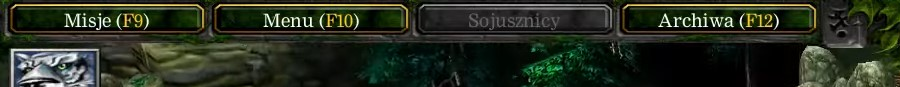
\includegraphics[width=1.0\textwidth]{images/ui/warcraft3_gorny_pasek_lewy.png}
    \caption{Lewa część paska z informacjami w grze Warcraft 3.}\label{fig:Warcraft3}
\end{figure}

\begin{figure}[htbp]
    \centering
    
\includegraphics[width=1.0\textwidth]{images/ui/warcraft3_gorny_pasek_prawy.png}
    \caption{Prawa część paska z informacjami w grze Warcraft 3.}\label{fig:Warcraft3}
\end{figure}